Up to now, our considerations were only focused on the operation times for making products and the reciepee of the final product. In this chapter, we will start complexifying our model by adding the setup time for machines. The setup time corresponds to the time in which the machine isn't used to actually produce one good but rather to "get ready" to do so. For instance, one machine has a "cold start" or may need some preparation like changing drills or configurations. We will see in this chapter that the setup time is actually a critical aspect of the production plant and that it drives the batch sizes in a very precise way. The figure (\ref{setup:gant_ex}) shows how the setup time impacts the production of a given batch.

\begin{figure}[h!]
    \centering
    \begin{tikzpicture}
        \draw[->] (0,0) node[left] {$i$} -- (7, 0);
        \draw (1.5, .75) node {$T_{si}$} ++(1.5, 0) node {$T_{oi}$};
        \draw[dotted] (1,0) rectangle (2, .5);
        \draw (2, 0) rectangle (4, .5);
        \draw (3, .25) node {$b_i$};

        \draw[decorate, decoration={brace, amplitude=10pt}] (4, -.1) -- (1, -.1);
        \draw (3.25, -1) node {$\dfrac{b_i}{T_{si} + b_iT_{oi}} = \mu_i(b_i)$};
    \end{tikzpicture}
    \caption{\label{setup:gant_ex}Simple example of batch production with setup time in GANT representation}
\end{figure}

Concerning the rate of production of mahcine $i$ as depicted in figure (\ref{setup:gant_ex}), a few considerations are to be made : (1) of course, if we set the setup time to be zero we get back with our previous formula $\mu_i = 1/T_{oi}$ ; (2) when $b_i\rightarrow\infty$, we also get that $\mu_i(b_i)\rightarrow\frac{1}{T_{oi}}$, this can be simply explain as the fact that, if we produce more and more products in one batch, the setup time (which is paid just once), becomes less and less significant with respect to the production time.

As far as the representation in terms of graph (bill of materials) is concerned, we will now fill the first element of the couple valuating transformations with the setup times for each machine as you can see in figure (\ref{setup:graph_setup}).

\begin{figure}[h!]
    \centering
    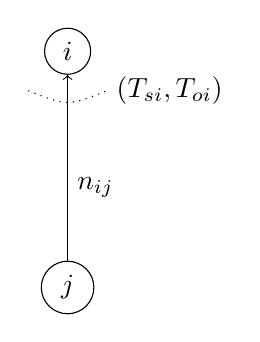
\begin{tikzpicture}
        \draw (0, 0) node[draw, circle] (i) {$i$} ++(0, -3) node[circle, draw] (j) {$j$};
        \draw[<-] (i) -- node[below right] {$n_{ij}$} (j);
        \draw[dotted] (-.5, -.5) .. controls (0, -.7) .. (.5, -.5) node[right] {$(T_{si}, T_{oi})$};
    \end{tikzpicture}
    \caption{\label{setup:graph_setup}Simple example of batch production with setup time in GANT representation}
\end{figure}

\section{Finding the bottleneck machine(s)}

But let's get back to our prior concerns : production rates. Of course the following fomrula still holds : \[ X_f^{max} = \min_i\left( \frac{\mu_i}{n_{if}} \right) \]As we did in the last chapter, we will consider setting the batch size as exactely $b_i = n_{if}b_f$ so that \[ X_f^{max} = \min_i\left( \frac{b_f}{T_{si} + T_{oi}b_fn_{if}} \right) \] which in trun is no longer a constant but rather a function of $b_f$. We will denote it as $X_f^{max}(b_f)$ not to forget it. The meaning of this is that now the maximum rate of production depends on the batch size we use with respect to the characteristics of the machines we use. And it is somehow logical since we know that producing batches of $1$ item would mean "paying" for the setup time for $1$ operation time whereas using batches of $10$ items would mean paying once the setup time for $10$ operation times ! As well, the overall production time is influenced by the setup times in a very simple way : \[ T_{prod}(b_f) = \max_{\mathcal P_k}\left( \sum_{i\in\mathcal P_k}(T_{si} + T_{oi}b_fn_{if}) \right) \]

\begin{wrapfigure}[16]{l}{5cm}
    \centering
    \begin{tikzpicture}
        \draw (0,0) node[draw, circle] (f) {$f$};
        \draw (-1, -2) node[draw, circle] (1) {$1$};
        \draw (-1, -4) node[draw, circle] (RM1) {$\vphantom{1}$};

        \draw (1, -2) node[draw, circle] (2) {$2$};
        \draw (1, -4) node[draw, circle] (3) {$3$};
        \draw (1, -6) node[draw, circle] (4) {$4$};
        \draw (1, -8) node[draw, circle] (RM2) {$\vphantom{1}$};

        \draw[->] (RM1) -- (1);
        \draw[->] (1) -- (f);

        \draw[->] (RM2) -- (4);
        \draw[->] (4) -- (3);
        \draw[->] (3) -- (2);
        \draw[->] (2) -- (f);

        \draw[dotted] (-.5, -.5) .. controls (0, -.7) .. (.5, -.5) node[right] {$(1, 1)$};
        \draw[dotted] (-1.5, -2.5) node[left] {$(1, 2)$} .. controls (-1, -2.7) .. (-.5, -2.5);
        
        \draw[dotted] (.5, -2.5) .. controls (1, -2.7) .. (1.5, -2.5) node[right] {$(10, 1)$};
        \draw[dotted] (.5, -4.5) .. controls (1, -4.7) .. (1.5, -4.5) node[right] {$(1, 1)$};
        \draw[dotted] (.5, -6.5) .. controls (1, -6.7) .. (1.5, -6.5) node[right] {$(1, 1)$};
    \end{tikzpicture}
    \caption{\label{setup:bill_of_mat1}Bill of material with setup time example}
\end{wrapfigure}

Let's have an example to better understand what it means to have a maximum production rate which depends on the batch size. Let's consider the bill of materials of figure (\ref{setup:bill_of_mat1}) and let's compute $X_f^{max}$. Note that when no $n_{if}$ coefficient is written, it is assumed to be $1$. 

Applying the given formula, we gen that
\[
    \begin{split}
        X_f^{max} &= \min_i\left( \frac{b_f}{1+1.b_f} ; \frac{b_f}{1+2.b_f} ; \frac{b_f}{10 + 1.b_f} ; \frac{b_f}{1+1.b_f} ; \frac{b_f}{1 + 1.b_f} \right)\\
                  &= \min_i\left( \frac{b_f}{1+1.b_f} ; \frac{b_f}{1+2.b_f} ; \frac{b_f}{10 + 1.b_f} \right)\\
                  &= \min_i\left( \frac{1}{1+2.b_f} ; \frac{1}{10 + 1.b_f} \right)
    \end{split}
\]

You may notice that in line 2 of these equations, we got rid of the first value because, in any case, we knew it was lower than the other ones since $1+1.b_f<1+2.b_f$ and $1+1.b_f<10+1.b_f$. The discussion now continues with respect to the machine $1$ and $2$ and we should look at figure (\ref{setup:bottleneck_dependent}) which plots the functions $b_f\mapsto 1+2b_f$ and $b_f\mapsto 10+b_f$. The bottleneck machine is then given by $\textrm{arg}\min_i\left(\frac{1}{1+2.b_f} ; \frac{1}{10 + 1.b_f}\right) = \textrm{arg}\max_i(1+2.b_f ; 10 + 1.b_f)$ which corresponds to the second machine (machine $2$) as long as the bacth size is less than $9$ and corresponds to the first machine (machine $1$) when $b_f > 9$. 

\begin{figure}[h!]
    \centering
    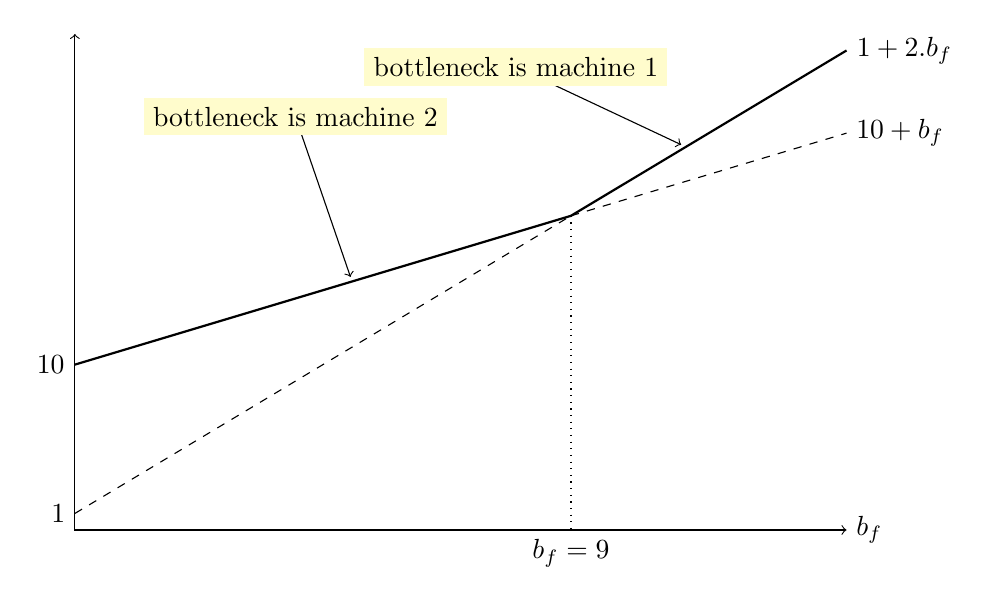
\begin{tikzpicture}[scale=0.7, yscale=0.3]
        \draw[<->] (0, 30) |- (14, 0) node[right] {$b_f$};

        \draw[thick] (0, 10) node[left] {$10$} -- (9, 19);
        \draw[dashed] (9, 19) -- (14, 24) node[right] {$10 + b_f$};
        \draw[->] (4, 25) node[fill=yellow!20] {bottleneck is machine $2$} -- (5, 15.3);

        \draw[dashed] (0, 1) node[left] {$1$} -- (9, 19);
        \draw[thick] (9,19) -- (14, 29) node [right] {$1+2.b_f$};
        \draw[->] (8, 28) node[fill=yellow!20] {bottleneck is machine $1$} -- (11, 23.3);

        \draw[dotted] (9, 19) -- (9,0) node[below] {$b_f=9$};
    \end{tikzpicture}
    \caption{\label{setup:bottleneck_dependent}Bottleneck machine depending on the batch size}
\end{figure}

Similarly, the production time for producing a batch of size $b_f$ can be computed as
\[
    \begin{split}
        T_{prod}(b_f) &= \max( (1+2.b_f) + (1 + 1.b_f) ; (1+1.b_f) + (1 + 1.b_f)\\&+ (10 + 1.b_f)+ (1 + 1.b_f) )\\
        &= \max(2+3.b_f ; 13 + 4.b_f)
    \end{split}
\]

\section{Controlling the production rate}

Let's get deeper with the interpretation of what have been said by looking at both figure (\ref{setup:production_rate_depends}) and (\ref{setup:production_time_depends}). The first figure shows a situation in which we would like compute the batch size of our production by imposing a certain production rate $X_f^*$ so that $X_f\ge X_f^*$. Solving this problem is, in fact, rather simple and can be done like so
\[
    \begin{split}
        X_f\ge X_f^* &\Leftrightarrow \min_i\left( \frac{b_f}{T_{si} + b_fT_{oi}n_{if}} \right) \ge X_f^*\\
            &\Leftrightarrow \frac{b_f}{T_{si} + b_fT_{oi}n_{if}} \ge X_f^*, \forall i\\
            &\Leftrightarrow b_f \ge X_f^*( T_{si} + T_{oi}b_fn_{if} )\\
            &\Leftrightarrow b_f \ge \frac{ X_f^*T_{si} }{ 1 - X_f^*T_{oi}n_{if} }, \forall i\\
            &\Leftrightarrow b_f \ge \max_i\left( \frac{ X_f^*T_{si} }{ 1 - X_f^*T_{oi}n_{if} } \right) = b_f^*
    \end{split}
\]
Notice that we used the fact that $1-X_f^*T_{oi}n_{if} \ge 0$ to go from the third line to the fourth one. This is true because it is equivalent to $ X_f^*\ge\frac{1}{T_{oi}n_{if}} $ which has to hold, otherwise, imposing $X_f^*$ would not be feasible. 

\begin{wrapfigure}[14]{l}{5cm}
    \centering
    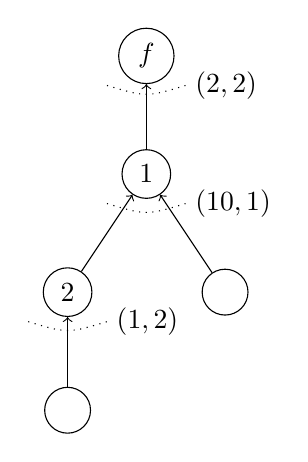
\begin{tikzpicture}[yscale=0.75]
        \draw (0,0) node[draw, circle] (f) {$f$};
        \draw (0,-2) node[draw, circle] (1) {$1$};
        \draw (-1,-4) node[draw, circle] (2) {$2$};
        \draw (-1,-6) node[draw, circle] (RM1) {$\vphantom{j}$};
        \draw (1,-4) node[draw, circle] (RM2) {$\vphantom{j}$};

        \draw[->] (1) -- (f);
        \draw[->] (2) -- (1);
        \draw[->] (RM1) -- (2);
        \draw[->] (RM2) -- (1);

        \draw[dotted] (-.5, -.5) .. controls (0, -.7) .. (.5, -.5) node[right] {$(2, 2)$};
        \draw[dotted] (-.5, -2.5) .. controls (0, -2.7) .. (.5, -2.5) node[right] {$(10, 1)$};
        \draw[dotted] (-1.5, -4.5) .. controls (-1, -4.7) .. (-.5, -4.5) node[right] {$(1, 2)$};
    \end{tikzpicture}
    \caption{\label{setup:bill_of_mat2}Bill of material}
\end{wrapfigure}

Let's take an example in order to see how we can play with these equations. Let's consider the bill of materials presented in figure (\ref{setup:bill_of_mat2}) and let us assume that we want to achieve a production rate of at least $X_f^* = 0.9 X_f^{max}(b_f^{max})$. For this example, we will assume that there is no upper bound for batch sizing so that $b_f^{max} = \infty$. It holds that \[ X_f^{max} = \min_i\left( \frac{1}{T_{oi}n_{if}} \right) = \min\left( \frac{1}{2} ; \frac{1}{1} ; \frac{1}{2} \right) = \frac{1}{2} \] which tells us that the bottleneck machines are the one denoted by $f$ and by $2$, and that the production we actually want to achieve is $X_f^* = .45$. That being said, we can now compute the minimum batch size we can use in order to fullfill this constraint. This is done lke so : \[ b_f^* = \max_i\left( \frac{.45\times 2}{1 - .45\times 2} ; \frac{.45\times 10}{1 - .45\times 1} ; \frac{.45\times 1}{1 - .45\times 2} \right) = 9 \]

Let's assume that we choose to use exactely $b_f^*$ as our batch size (any greater size is actually also valid) to produce at rate $X_f^*$, exactely. Then, one cycle should lasts \[ D^* = \frac{b_f}{X_f^*}=\frac{9}{.45} = 20 \] And let's have a look at the GANT diagram given by these parameters in figure (\ref{setup:gant_mat2}). We can see that the bottleneck machine is the machine $f$ and that the machine $2$ is no more a bottleneck as we had originally planned. That is because the bottleneck machine actually depends on the batch size we use. When we firstly computed the bottleneck machines (when we computed $X_f^{max}$), we did it assuming that the batch size was the maximum one, which is no longer true. To make this even more clear, let's deal with the case where we want, with the same production plant, produce at a rate of $X_f^*=.3$ instead of $0.45$. But let us still use batches of $9$. 

First, let's make sure that it is possible to use $b_f = 9$ by computing the lowest batch size we can use with respect to the constraint $X_f\ge .3$ :
\[
    \begin{split}
        b_f^* &= \max\left( \frac{.3\times 2}{1 - .3\times 2} ; \frac{.3\times 10}{1 - .3\times 1} ; \frac{.3\times 1}{1-.3\times 2} \right)\\
        &= \max\left( \frac{3}{2} ; \frac{30}{7} ; \frac{3}{4} \right)\\
        &= \frac{30}{7} \approx 4
    \end{split}
\]
This tells us two things : (1) that the batch size has to be greater than $4$ (so we can use $9$ while respecting our constraints) ; (2) that if we use $b_f = b_f^*$, the bottleneck machine will be machine $1$. However, and as discussed, the GANT diagram in figure (\ref{setup:gant_mat2_2}), the bottleneck machine is actually still the machine $f$ if we use $9$ as our batch size. The production cycle is computed as always by $D^* = \frac{9}{.3} = 30$. 

\begin{figure}[h!]
    \centering
    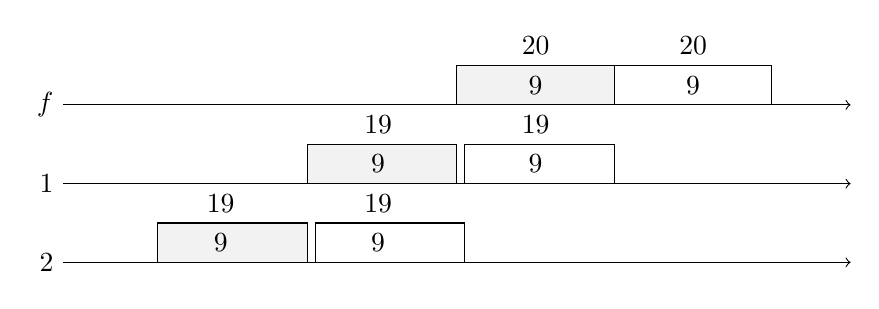
\begin{tikzpicture}
        \draw[->] (0,0) node[left] {$f$} -- (10, 0);
        \draw (7, 0) rectangle (9, .5);
        \draw[fill=gray!10] (5, 0) rectangle (7, .5);
        \draw (8, .75) node {$20$} ++(-2, 0) node {$20$};
        \draw (8, .25) node {$9$} ++(-2, 0) node {$9$};

        \draw[->] (0,-1) node[left] {$1$} -- (10, -1);
        \draw (7-1.9, -1) rectangle (7, -.5);
        \draw[fill=gray!10] (5-1.9, -1) rectangle (5, -.5);
        \draw (6, -.25) node {$19$} ++(-2, 0) node {$19$};
        \draw (6, -.75) node {$9$} ++(-2, 0) node {$9$};

        \draw[->] (0,-2) node[left] {$2$} -- (10, -2);
        \draw[fill=gray!10] (5-1.9-1.9, -2) rectangle (5-1.9, -1.5);
        \draw (7-1.9-1.9, -2) rectangle (7-1.9, -1.5);
        \draw (4, -1.25) node {$19$} ++(-2, 0) node {$19$};
        \draw (4, -1.75) node {$9$} ++(-2, 0) node {$9$};
    \end{tikzpicture}
    \caption{\label{setup:gant_mat2}GANT diagram when $X_f^*=0.45$ and batch size is $b_f=b_f^*=9$}
    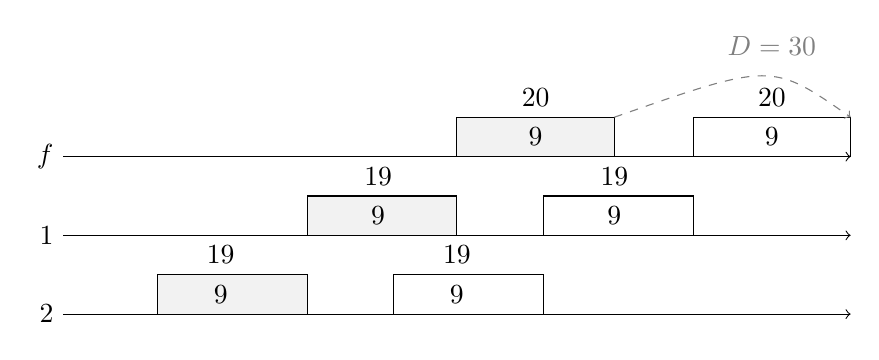
\begin{tikzpicture}
        \draw[->] (0,0) node[left] {$f$} -- (10, 0);
        \draw (8, 0) rectangle (10, .5);
        \draw[fill=gray!10] (5, 0) rectangle (7, .5);
        \draw (9, .75) node {$20$} ++(-3, 0) node {$20$};
        \draw (9, .25) node {$9$} ++(-3, 0) node {$9$};

        \draw[->] (0,-1) node[left] {$1$} -- (10, -1);
        \draw (8-1.9, -1) rectangle (8, -.5);
        \draw[fill=gray!10] (5-1.9, -1) rectangle (5, -.5);
        \draw (7, -.25) node {$19$} ++(-3, 0) node {$19$};
        \draw (7, -.75) node {$9$} ++(-3, 0) node {$9$};

        \draw[->] (0,-2) node[left] {$2$} -- (10, -2);
        \draw[fill=gray!10] (5-1.9-1.9, -2) rectangle (5-1.9, -1.5);
        \draw (8-1.9-1.9, -2) rectangle (8-1.9, -1.5);
        \draw (5, -1.25) node {$19$} ++(-3, 0) node {$19$};
        \draw (5, -1.75) node {$9$} ++(-3, 0) node {$9$};

        \draw[dashed, gray, ->] (7, .5) .. controls (9, 1.2) .. (10, .5);
        \draw[gray] (9, 1.4) node {$D = 30$};
    \end{tikzpicture}
    \caption{\label{setup:gant_mat2_2}GANT diagram when $X_f^*=0.3$ and batch size is $b_f=9$}
\end{figure}

\begin{figure}[p]
    \centering
    \begin{tikzpicture}[scale=1.1, yscale=0.3, xscale=.4]
        \draw[<->] (0, 20) node[above] {$X_f^{max}(b_f)$} |- (30, 0) node[right] {$b_f$};
        
        \draw (0,0) .. controls (5, 6) .. (10, 8);
        \draw (10.1,8.1) .. controls (15, 12) .. (20, 14);
        \draw (20.1,14.1) .. controls (25, 17.7) .. (30, 18);

        \draw[gray] (15, 20.5) node {$ X_f^{max}(\infty) = \min_i\left( \dfrac{1}{T_{oi}n_{if}} \right) $};
        \draw[dashed, gray] (0, 18.2) -- (30, 18.2);

        \draw[dotted] (0, 12) node[left] {$X_f^*$} -| (15, 0) node[below] {$b_f^*\rightarrow$};
    \end{tikzpicture}
    \caption{\label{setup:production_rate_depends}How the production rate depends on the batch size}
    \begin{tikzpicture}[scale=1.1, yscale=0.3, xscale=.4]
        \draw[<->] (0, 20) node[above] {$T_{prod}(b_f)$} |- (30, 0) node[right] {$b_f$};

        \draw (1, 4) -- (8, 10);
        \draw (8, 10) -- (18, 13);
        \draw (18, 13) -- (30, 20);

        \draw[dotted] (1, 0) node[below] {$b_f = 1$} |- (0, 4) node[left] {$T_{si}$};
        \draw[dotted] (0, 10.4) node[left] {$\bar T$} -| (9, 0) node[below] {$\bar b_f$};
    \end{tikzpicture}
    \caption{\label{setup:production_time_depends}How the production time depends on the batch size}
\end{figure}

\section{Controlling the production time}

We now can satisfy constraints on the production rate, which is a good thing. However, production plants often encounter another kind of constraints which is linked to the production time. In this section, we will focus on what happens when we impose that the overall production time must be lower than a certain duration. More formally, we impose that $T_{prod}\le\bar T$. The computation is similar to what have been done so far and is given by :
\[
    \begin{split}
        T_{prod}\le\bar T
            &\Leftrightarrow \max_{\mathcal P_k}\left( \sum_{i\in\mathcal P_k} ( T_{si} + T_{oi}b_fn_{if} ) \right)\le\bar T\\
            &\Leftrightarrow \sum_{i\in\mathcal P_k} T_{si} + b_f\sum_{i\in\mathcal P_k}T_{oi}n_{if} \le\bar T, \forall\mathcal P_k\\
            &\Leftrightarrow b_f\le \frac{\bar T - \sum_{i\in\mathcal P_k}T_{si}}{\sum_{i\in\mathcal P_k} T_{oi}n_{if}}, \forall\mathcal P_k\\
            &\Leftrightarrow b_f\le\min_{\mathcal P_k}\left( \frac{\bar T - \sum_{i\in\mathcal P_k} T_{si}}{\sum_{i\in\mathcal P_k}T_{oi}n_{if}} \right) = \bar b_f
    \end{split}
\]

\begin{wrapfigure}[19]{r}{5cm}
    \centering
    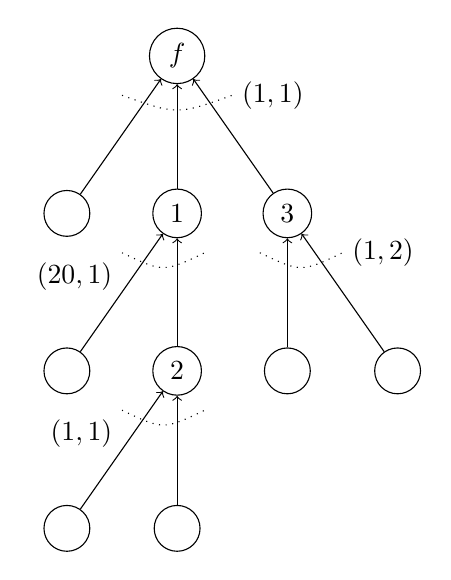
\begin{tikzpicture}[xscale=0.7]
        \draw (0,0) node[circle, draw] (f) {$f$};
        \draw (0,-2) node[circle, draw] (1) {$1$};
        \draw (0,-4) node[circle, draw] (2) {$2$};
        \draw (0,-6) node[circle, draw] (RM4) {$\vphantom{j}$};
        \draw (-2, -2) node[circle, draw] (RM1) {$\vphantom{j}$};
        \draw (-2, -4) node[circle, draw] (RM2) {$\vphantom{j}$};
        \draw (-2, -6) node[circle, draw] (RM3) {$\vphantom{j}$};
        \draw (2, -2) node[circle, draw] (3) {$3$};
        \draw (2, -4) node[circle, draw] (RM5) {$\vphantom{j}$};
        \draw (4, -4) node[circle, draw] (RM6) {$\vphantom{j}$};

        \draw[->] (RM1) -- (f);
        \draw[->] (RM2) -- (1);
        \draw[->] (RM3) -- (2);
        \draw[->] (RM4) -- (2);
        \draw[->] (1) -- (f);
        \draw[->] (3) -- (f);
        \draw[->] (2) -- (1);
        \draw[->] (RM5) -- (3);
        \draw[->] (RM6) -- (3);

        \draw[dotted] (-1, -.5) .. controls (0, -.75) .. (1, -.5) node[right] {$(1, 1)$};
        \draw[dotted] (-1, -2.5) node[below left] {$(20,1)$} .. controls (-.25, -2.75) .. (.5, -2.5);
        \draw[dotted] (-1, -4.5) node[below left] {$(1,1)$} .. controls (-.25, -4.75) .. (.5, -4.5);
        \draw[dotted] (1.5, -2.5) .. controls (2.25, -2.75) .. (3, -2.5) node[right] {$(1,2)$};
    \end{tikzpicture}
    \caption{\label{setup:bill_of_mat3}Bill of materials}
\end{wrapfigure}

Let's take another example considering figure (\ref{setup:bill_of_mat3}) to introduce how we can handle situations in which we both have a condition on production time and on production rate. To do that, consider the following problem : finding $b_f$ subject to the constraints : \[
    \begin{cases}
        X_f \ge X_f^*\\
        T_{prod} \le \bar T
    \end{cases}
    \textrm{ with }
    X_f^* = 0.8\times X_f^{max}(b_f^{max})
    \textrm{ and }
    \bar T = 10\times T_{prod}(1)
\]
Let's first compute the inputs of our problem which are $X_f^{max}(b_f^{max})$ and $T_{prod}(1)$. Since no maximum batch size has been given, we will consider that $b_f^{max}=\infty$ so that \[ X_f^{max}(b_f^{max}) = \min_i\left( \frac{1}{T_{oi}n_{if}} \right) = \min\left( \frac{1}{1} ; \frac{1}{2} \right) = \frac{1}{2} \] and \[ T_{prod}(1) = \max_{\mathcal P_k}( 25 ; 5 ) = 25 \] which gives us the values we wanted : $X_f^* = 0.4$ and $T_{prod} = 250$.

Considering the first constraint (on the production rate), we can compute a lower bound for our batch size :
\[
    \begin{split}
        b_f^* &= \max_i\left( \frac{X_f^*T_{si}}{1-X_f^*T_{oi}n_{if}} \right) =
        \max\left( \frac{.4\times 1}{1-.4\times 1\times 1} ; \frac{.4\times 20}{1-.4\times 1\times 1} ; \frac{.4\times 1}{1-.4\times 1\times 1} ; \frac{.4\times 1}{1-.4\times 2\times 1} \right)\\
        &= \max\left( \frac 23, \frac{40}3 ; \frac 23 ; 2 \right) \approx 13.33
    \end{split}
\]
Using the other constraint (on the production time), we can then compute an upper bound for the batch size :
\[
    \bar b_f = \min_{\mathcal P_k}\left( \frac{\bar T - \sum_{i\in\mathcal P_k} T_{si}}{\sum_{i\in\mathcal P_k}T_{oi}n_{if}} \right) = \min\left( \frac{250 - 22}{3} ; \frac{250 - 2}{3} \right) = 76
\]

\begin{wrapfigure}[10]{r}{4cm}
    \centering
    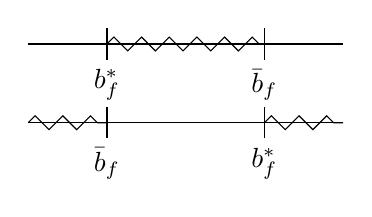
\begin{tikzpicture}[xscale=.5]
        \draw (0,0) -- (8, 0);
        \draw (0,-1) -- (8,-1);

        \draw[decorate,decoration=zigzag] (2,0) -- (6,0);
        \draw (2,.2) -- (2,-.2) node[below] {$b_f^*$};
        \draw (6,.2) -- (6,-.2) node[below] {$\bar b_f$};

        \draw[decorate,decoration=zigzag] (0,-1) -- (2,-1);
        \draw[decorate,decoration=zigzag] (6,-1) -- (8,-1);
        \draw (2,-.8) -- (2,-1.2) node[below] {$\bar b_f$};
        \draw (6,-.8) -- (6,-1.2) node[below] {$b_f^*$};
    \end{tikzpicture}
    \caption{\label{setup:bounds}Batch size}
\end{wrapfigure}

Which gives us the final solution : \[ b_f^* = 14 \le b_f \le 76 = \bar b_f \]
Of course, it is possible to write infeasible constraints which would lead to having $\bar b_f < b_f^*$. This situation is depicted in figure (\ref{setup:bounds}). If such a situation were to happen, the way of solving it is to decrease the setup time which means either (1) numerically decreasing the setup time (buying new machines for example) or buy masking the setup time. 